\documentclass[10pt,a4paper]{article}

%%%%%%%%%%%%%%%%%%%%%%%%%%%
% MODIFY:

\newcommand{\authorA}{Ahmad Bin Qasim (03693345)}
\newcommand{\authorB}{Kaan Atukalp (03709123)}
\newcommand{\authorC}{Martin Meinel (03710370)}
\newcommand{\groupNumber}{H} % - YOUR GROUP NUMBER
\newcommand{\exerciseNumber}{5} % - THE NUMBER OF THE EXERCISE
\newcommand{\sourceCodeLink}{https://gitlab.lrz.de/ga53rog/praktikum-ml-crowd}

\newcommand{\workPerAuthor}{
\authorA&Task 1&33\%\\
      &Task 2&33\%\\
      &Task 3&33\%\\
      &Task 4&33\%\\
      & Task 5&33\%\\
      \hline
\authorB&Task 1&33\%\\
      &Task 2&33\%\\
      &Task 3&33\%\\
      &Task 4&33\%\\
      & Task 5&33\%\\
      \hline
\authorC&Task 1&33\%\\
      &Task 2&33\%\\
      &Task 3&33\%\\
      &Task 4&33\%\\
      & Task 5&33\%\\
}

%%%%%%%%%%%%%%%%%%%%%%%%%%%

%%
% imports for the exercise sheets
%

\usepackage[utf8]{inputenc}
\usepackage{amsmath}
\usepackage{amsfonts}
\usepackage{amssymb}

\usepackage[yyyymmdd]{datetime}
\renewcommand{\dateseparator}{--}

\usepackage[left=2cm,right=2cm,top=3cm,bottom=3cm]{geometry}

\usepackage{hyperref}

\usepackage{amsthm}
\newtheorem{lem}{Lemma}
\newtheorem{thm}{Theorem}
\newtheorem{cor}{Corollary}
\newtheorem{rem}{Remark}
\newtheorem{definition}{Definition}
\newtheorem{ter}{Terminology}

\usepackage{graphicx}

\newcommand{\M}{\mathcal{M}}
\newcommand{\N}{\mathcal{N}}
\newcommand{\K}{\mathcal{K}}
\newcommand{\SPDk}{\mathbb{P}^k}
\newcommand{\vol}{\text{vol}}

\newcommand{\Figref}[1]{Figure~\ref{#1}}
\newcommand{\figref}[1]{figure~\ref{#1}}
\newcommand{\Eqnref}[1]{Equation~(\eqref{#1})}
\newcommand{\eqnref}[1]{equation~(\eqref{#1})}

\usepackage{float}
\usepackage{tabularx}
\usepackage{subcaption}
\usepackage{mwe}

\usepackage{fancyhdr}
\pagestyle{fancy}

\usepackage{totcount}
\newtotcounter{taskCounter}
\newtotcounter{pointCounter}
\newenvironment{task}[1]{\noindent\stepcounter{taskCounter}\textbf{Report on task #1}\smallbreak\hrule\smallbreak}{\smallbreak\hrule\bigbreak}


\title{Report for exercise \exerciseNumber~from group~\groupNumber}

\makeatletter
\let\thetitle\@title
\let\theauthor\@author
\let\thedate\@date
\makeatother

\providecommand{\versiondate}{\today}

\lhead{Exercise sheet \exerciseNumber}
\chead{Master Praktikum: Modelling and Simulation of Crowds WS2019/20}
\rhead{TUM}
\lfoot{Report of Group \groupNumber}
\cfoot{\thepage}
\rfoot{Last compiled: \versiondate}
\renewcommand{\headrulewidth}{0.4pt}
\renewcommand{\footrulewidth}{0.4pt}

\newcommand{\frontpage}{
\begin{center}
\textbf{\thetitle}\\~\\
\end{center}
\begin{table}[H]
\begin{tabular}{ll}
Tasks addressed:&\total{taskCounter}\\
Authors:&\authorA\\
&\authorB\\
&\authorC\\
Last compiled:&\versiondate\\
Source code:&\sourceCodeLink
\end{tabular}
\end{table}
\vfill
The work on tasks was divided in the following way:
\begin{table}[H]
\begin{tabularx}{\textwidth}{X|p{2cm}|p{2cm}}
\workPerAuthor
\end{tabularx}
\end{table}
\newpage
}

\begin{document}

\frontpage

\begin{task}{1, Approximating functions}
Part 1: \bigbreak
For part 1 we loaded the linear data from the "linear\_function.txt" file and tried to approximate the function linearly. We used a linear regression model to minimize the mean square error. For this problem there exists a closed form solution to compute the matrix A which contains the parameters to map the input to the output with a minimal mean square error to the original function, we want to approximate. 
The mean squares error problem is defined by following equation:
\begin{equation*}
\min_{\hat{f}}e(\hat{f}) = \min_{\hat{f}}||F-\hat{f}(X)||^2 = \min_{A}||F-XA^T||^2
\end{equation*}
Figure \ref{fig:task1_1} shows the original linear data in blue and its linear approximation in orange. It can be easily seen that all data points are laying on the linear straight which was computed with the closed form solution. The data is linear so the function can be approximated perfectly.
\begin{figure}[H]
\centering
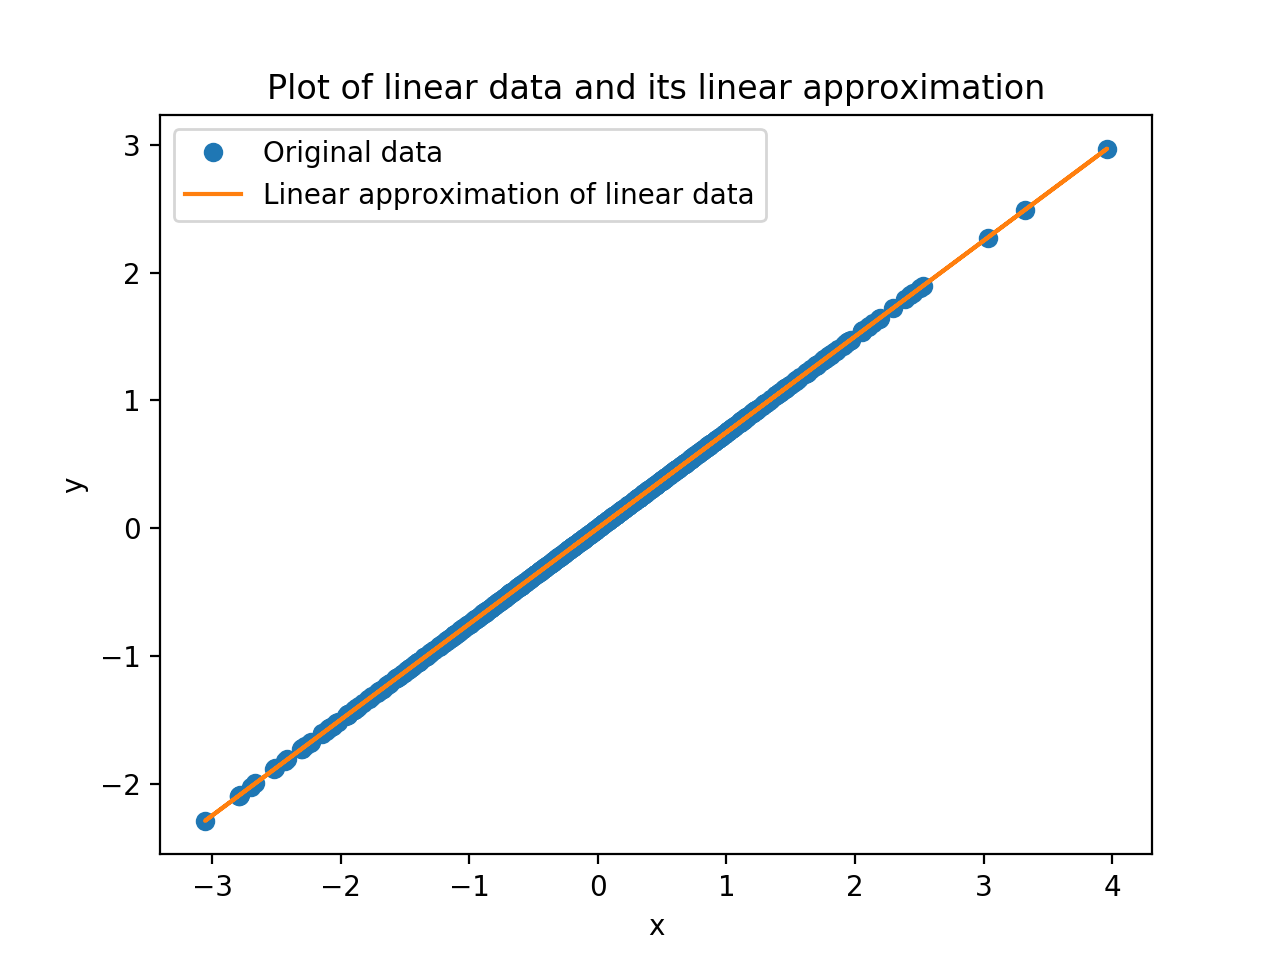
\includegraphics[width=0.7\textwidth]{../plots/task1_part1.png}
\caption{Plot of the linear data and its linear approximation}
\label{fig:task1_1}
\end{figure}
Part 2: \\
In the second part we use a nonlinear dataset from the "nonlinear\_function.txt" file and tried to approximate the function in a linear way again.
Figure \ref{fig:task1_2} shows then original data in blue again. The linear approximation of the function is  shown in orange. It can be easily seen that the linear approximation fits very bad. The reason for that is that the function is nonlinear and we try to approximate it linearly.
\begin{figure}[H]
\centering
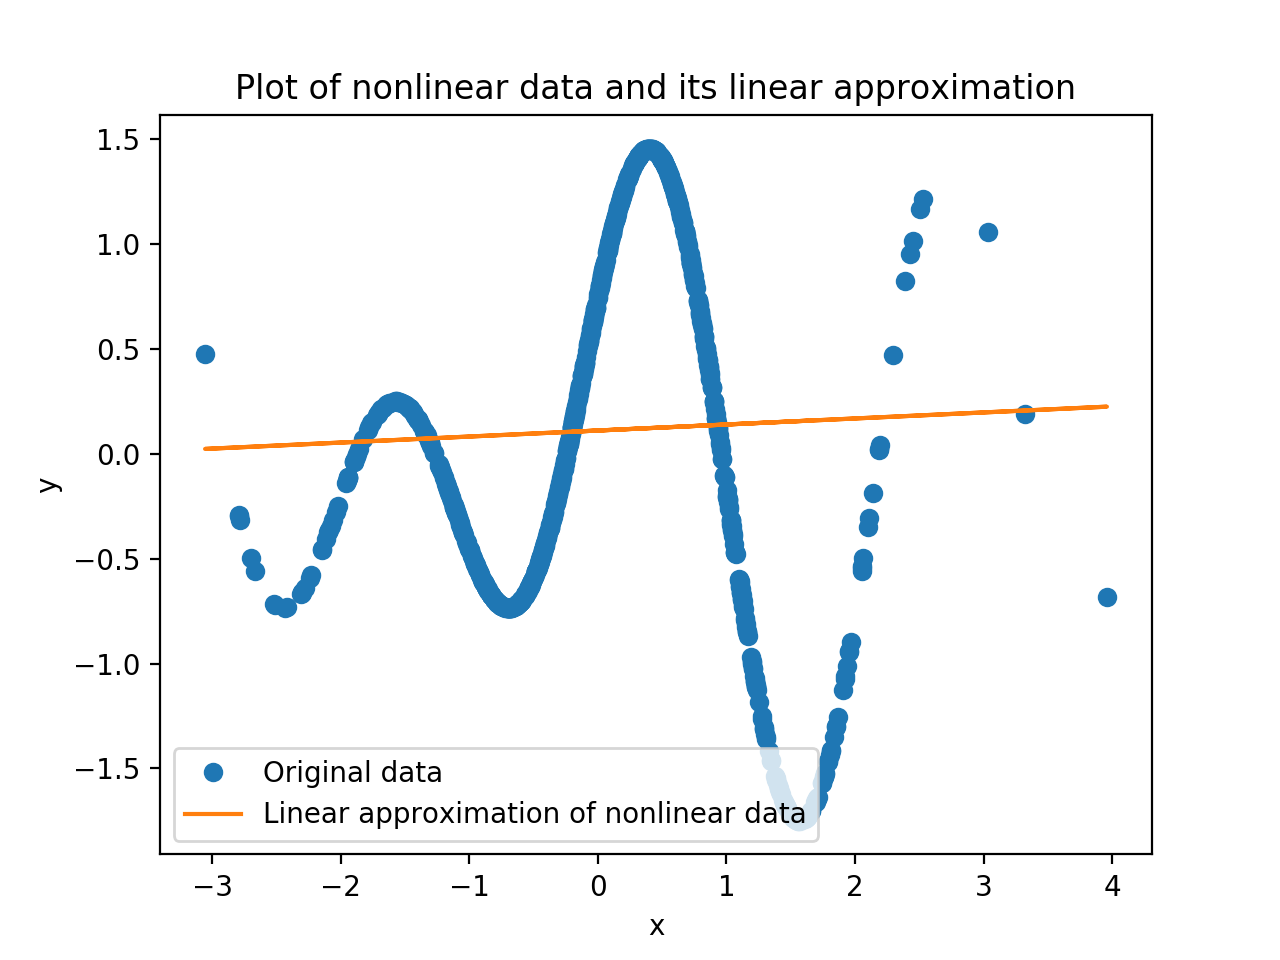
\includegraphics[width=0.7\textwidth]{../plots/task1_part2.png}
\caption{Nonlinear data and its linear approximation}
\label{fig:task1_2}
\end{figure}
Part 3: \\
After we tried to approximate the nonlinear dataset with a linear function in part 2, we now try to approximate the unknown nonlinear function with a combination of radial basis function:
\begin{equation*}
	\phi_l(x) = \exp(-||x_l -x||^2/\epsilon^2)
\end{equation*}
$x_l$ is the center of the basis function and usually just a randon point of the data set. There is one $x_l$ for each radial basis function. We have to choose how many basis functions L  we use to approximate the nonlinear function. Besides, we have to choose $\epsilon$ appropriately.
Figure \ref{fig:task1_3} shows the original data in blue and the approximated function which makes use of radial basis functions in orange. It can be easily seen that the approximation is by far better than the linear approximation of part 2. \\ In general the approximation fits the original function quite well.
We chose $\epsilon$ according to the $\epsilon$ in the diffusion maps task of the previous exercise sheet. This means we computed the distance matrix among all the x values and took the maximum value for $\epsilon$. This meaximum value is multiplied by 0.05. Besides, we use $L=15$ radial basis functions for the nonlinear approximation.
\begin{figure}[H]
\centering
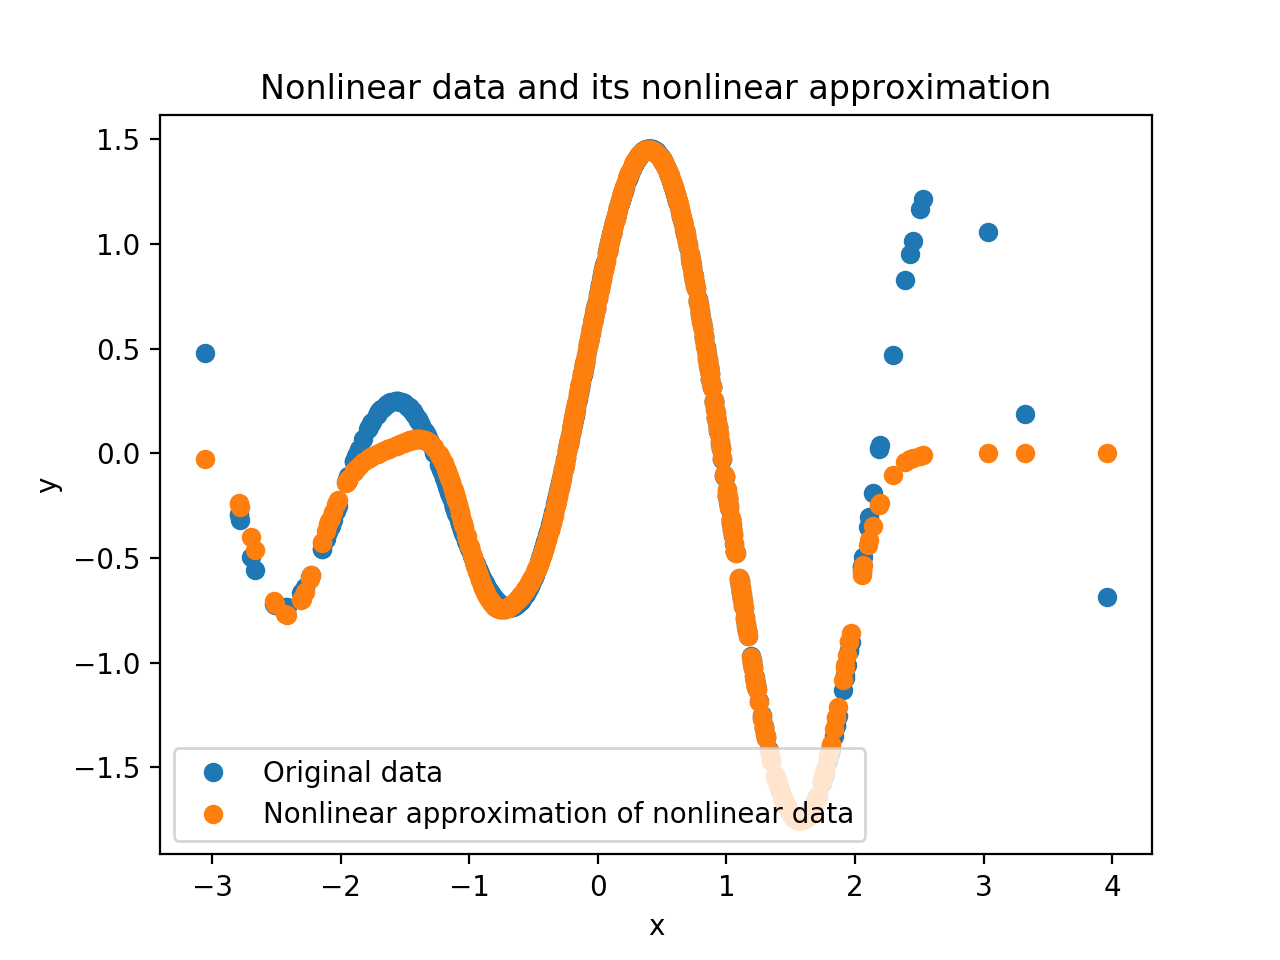
\includegraphics[width=0.7\textwidth]{../plots/task1_part3_eps.png}
\caption{Nonlinear data and its nonlinear approximation with radial basis functions}
\label{fig:task1_3}
\end{figure}
It is not a good idea to use radial basis functions to approximate a linear function such as the linear data set of A. You can use the radial basis functions to approximate a linear data set, but you should use a linear approximator, because the computational cost of the radial basis function is higher due to the fact that the distance matrix for all x has to be computed to determinate $\epsilon$. Besides the parameters of L and $\epsilon$ have to be chosen appropiately to obtain a good approximation.
\end{task}

\begin{task}{2, First step of a single pedestrian}
Part 1: \\
We use the pandas read\_csv function to read the text files containing two dimensional x0 and x1 data. We estimate the vector fields $v^{(k)}$ for each x0, using the finite-difference formula, given hereby:
\begin{equation*}
\hat{v}^{(k)} = \frac{x_1^{(k)} - x_0^{(k)}}{\Delta t}
\end{equation*}
Then we approximate the matrix $A$ such that:
\begin{equation*}
v(x_0^{(k)}) = v^{(k)} = Ax_0^{(k)}
\end{equation*}
An interesting thing to note is that, bias b is not added in this equation. This will have implications to the prediction later on. It will be mentioned in part 3.

For this purpose, we use the linear approximator implementation from task 1. As mentioned before the goal is to estimate the matrix $A$, such that the mean square error is minimized. This can be represented through the following equation:
\begin{equation*}
\min_{\hat{f}}e(\hat{f}) = \min_{\hat{f}}||F-\hat{f}(X)||^2 = \min_{A}||F-XA^T||^2
\end{equation*} \\

Part 2: \\
After fitting the linear approximator, we predict the vector fields, $\hat{v}^{(k)}$ for each x0. Then we use $\hat{v}^{(k)}$ with $\Delta t = 0.1$ to calculate $\hat{x1}^{(k)}$ using the formula.
\begin{equation*}
\hat{x1}^{(k)} = \hat{v}^{(k)}\Delta t + x0^{(k)}
\end{equation*}
We compare $x1^{(k)}$ and $\hat{x1}^{(k)}$ using the mean squared error formula and obtain the value of: 1.0532185339804091e-13 \\\\
Part 3: \\
We set $x0=(10, 10)^{(0)}$ and then estimate $\hat{v}^{(0)}$. We calculate $\hat{x1}^{(0)}$ using the equation given in part 2. Then using the corresponding $\hat{x1}^{(k-1)}$, we calculate the vector field $\hat{v}^{(k)}$ for it. We repeat this process for $T = 100$. We use steps of $\Delta t = 0.1$, so the total number of iterations are $\frac{T}{\Delta t} = 1000$. 
As seen in the figure \ref{fig:task2_3}, the motion stops at (0,0). We think that reason for this is that, we do not add bias term b to the linear approximator equation. Hence when $x=0$, then the matrix A has no effect on $\hat{x}$.

\begin{figure}[H]
\centering
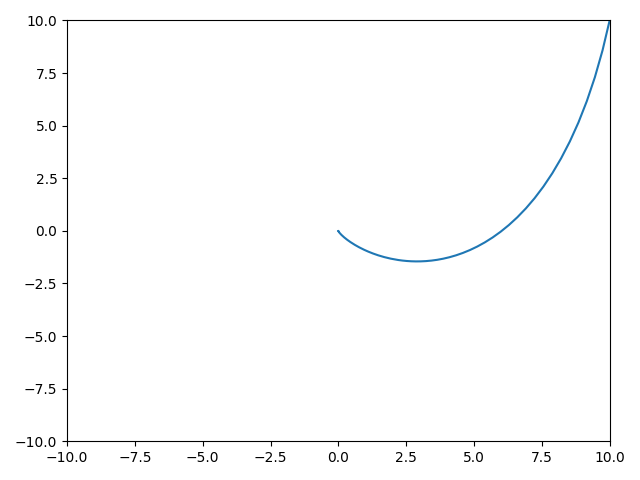
\includegraphics[width=0.7\textwidth]{../plots/task2_part3.png}
\caption{Trajectory of the motion}
\label{fig:task2_3}
\end{figure}

The phase portrait is given hereby:
\begin{figure}[H]
\centering
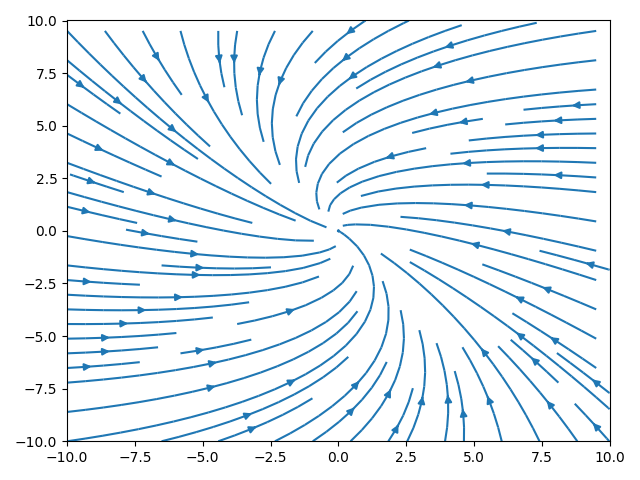
\includegraphics[width=0.7\textwidth]{../plots/task2_part3_phase.png}
\caption{The phase portrait}
\label{fig:task2_3_phase}
\end{figure}

\end{task}

\begin{task}{3, Approximating nonlinear vector fields}
Part 1: \\
At first we compute a vector $\hat{v}^{(k)}$ for every intial point $x_0^{(k)}$ with the equation:
\begin{equation*}
\hat{v}^{(k)} = \frac{x_1^{(k)} -x_0^{(k)}}{\Delta t}
\end{equation*}
We use the linear approximator to approximate the vector field and obtain A. After getting A we approximate $\hat{x_1^{(k)}}$ and compute the mean squarred error between the aproximated and the known end points for a chosen $\Delta t = 0.5$.
The mean squared error is 75.54.\bigbreak
Part 2: \\
Part 2 is similar to part 1, but this time we approximate the vector field with radial basis functions. We choose $L=10$ and take  for $\epsilon$ the biggest value of a distance matrix between all initial points $x_0$.
The mean squared error is 0.24. \\
The mean squarred error is extremely low, so the performance of the nonlinear approximator is very good. Consequently you can see that the vector field is nonlinear. Otherwise the mean squared error of the linear approximation would be lower.
You can see that the difference between both mean squared errors is high, because the mean squared error of the nonlinear approximated vector field is very low. \bigbreak
Part 3: \\
We use for this part the nonlinear approximator, because in our opinion the vector field is nonlinear. The nonlinear approximator shows better performance in comparison to the lineaer approximator. We use the approximated vector field to solve  the system for a larger time with all intitial points $x_0$.\\
Figure \ref{fig:task3_part3} shows the end state of the system. You can see several steady states. The steady states are at the following coordinates: \bigbreak
\begin{tabular}{|l|c|c|c|c|}
\hline
x-coordinate of steady state& -2.92&3.22&3.65&-4.26\\
y- coordinate of steady state& 3.13&1.85&-1.27&-3.65\\
\hline
\end{tabular}
\begin{figure}[H]
\centering
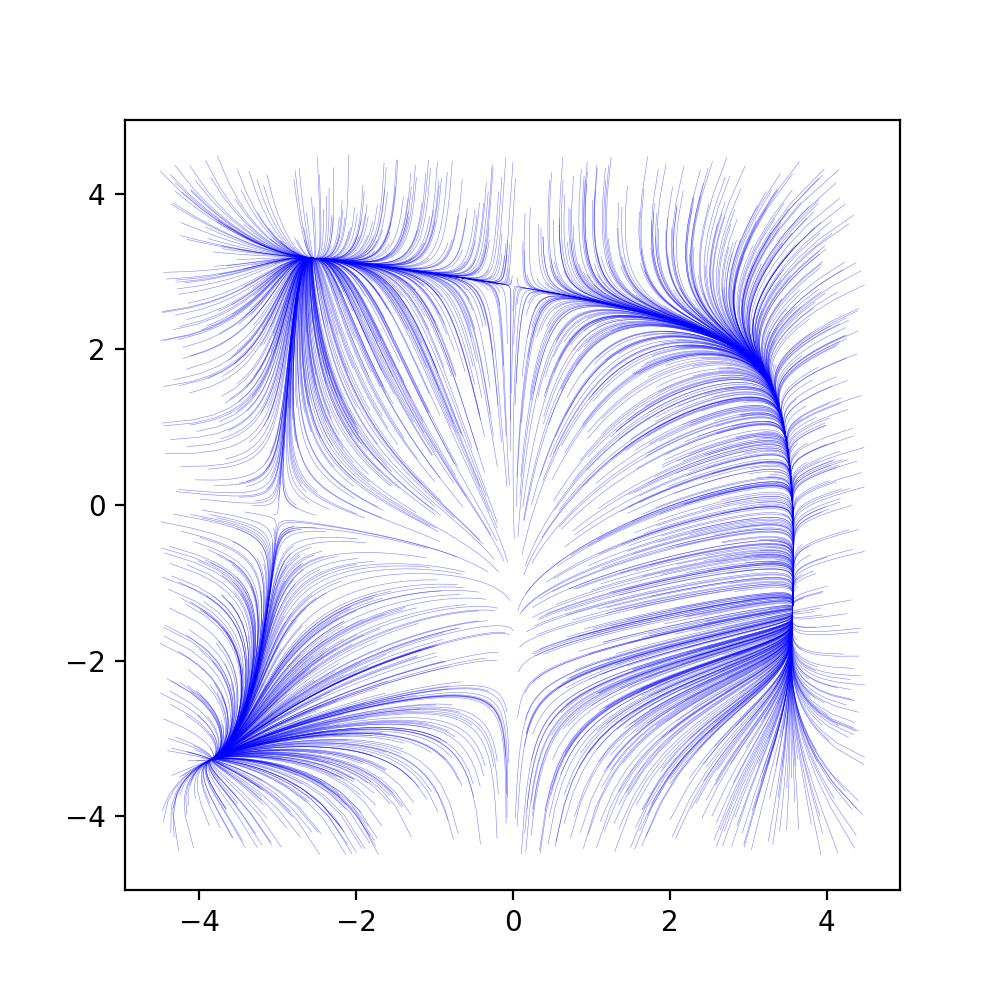
\includegraphics[width=0.7\textwidth]{../plots/task3_part3.png}
\caption{Predictions of $x_1$ for a larger time given initial points $x_0$}
\label{fig:task3_part3}
\end{figure}

\end{task}
\begin{task}{4, Obstacle avoidance}
Pedestrians can avoid obstacles, using Dijkstras algorithm. See figure.
\end{task}
\begin{task}{5, Tests}
\begin{enumerate}
\item[TEST1:] RiMEA scenario 1 (straight line, ignore premovement time)\\
- not done, but citing RiMEA guidelines -
\item[TEST2:] RiMEA scenario 4 (fundamental diagram, be careful with periodic boundary conditions).\\
- test successful - 
\item[TEST3:] RiMEA scenario 6 (movement around a corner).\\
- test successful - 
\item[TEST4:] RiMEA scenario\\
- test successful - 
\end{enumerate}
\end{task}



\end{document}